\chapter{Analyse}\label{sec:analyse}

\section{Systemsekvensdiagram}
\todo{write stuff about SSD}
\begin{figure}
    \centering
    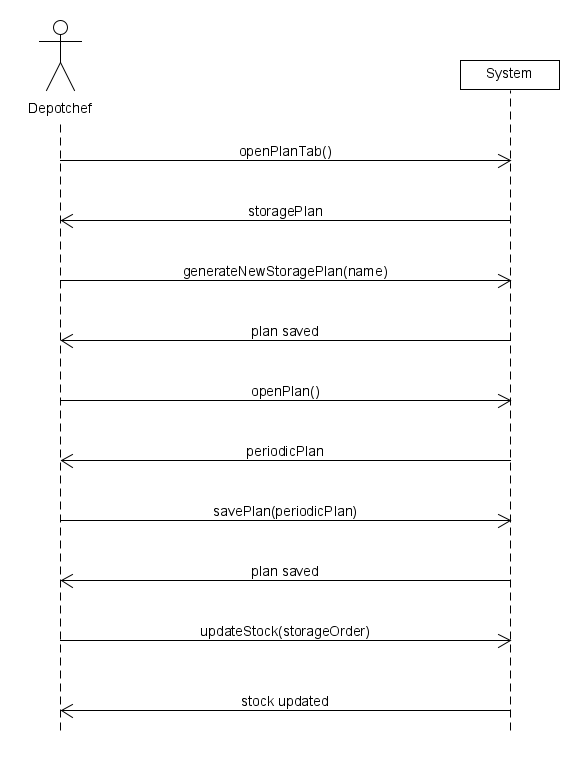
\includegraphics[width=50mm,scale=0.5]{figures/analyse/SSD.png}
    \caption{Systemsekvensdiagram}
    \label{fig:ssd}
\end{figure} 

\section{test til SSD}

SSD-diagrammet adresserer, hvordan brugeren og systemet kommunikerer frem og tilbage. Dette SSD-diagram er lavet ud fra Fully Dressed Use Case, automatisk lagerstyring.

 Her ses det, at depotchef Niels Thomas er såfremt den eneste, som benytter systemet. Som det første åbner Niels Thomas den nuværede plan for lageret, hvorefter vil systemet give den nuværende lager plan. 

Når åbnet, kan Niels Thomas generere en ny lager plan (generateNewStoragePlan(name)), samt navengive planen. Denne funktion generer en plan, basseret på salgsdata, produktets popularitet og kommende produkter. Når planen er genereret, vil den blive ved med at oprette storageOrders, baseret på den oprettede plan. 
Hvis planen såfremt har brug for ændring, skal du oprette en ny plan, åben den og herefter anvende dine brugerdefinerede ændringer. Et eksempel kunne være, du ville have 20 isbåde istedet for 10, herefter gemmer du planen og storageOrders er oprettet automatisk på ubestemt tid. 


\section{Operationskontrakt}
\todo{write stuff about operationskontrakt}
%remember to talk about the autogeneration continuation process thing algorithm stuff :) 

\begin{center}
    \begin{longtable}{ |p{360pt}| }
        \hline
        \textbf{Operationskontrakt}
        \\
        \noindent\fbox{%
            \parbox{4.88in}{%
                \textbf{Operation:} openPlanTab() \\ Åbner planfanen i programmet
                
            }%
        }

        \noindent\fbox{%
            \parbox{4.88in}{%
                \textbf{Operation:} generateNewStoragePlan(name) \\ 
                Use Case: Bestil Varer \\

                Præ-betingelser: en instans af productMap eksisterer \\

                Post-betingelser: \\
                - sp.name blev sat til name \\
                - En instans af PeriodicPlan blev oprettet \\
                - pp.period blev sat til period \\
                - en instans af sOrder blev oprettet \\
                - pp blev associeret med product og sOrder \\
                - p blev associeret med supplier og productLine \\
                - sOrder blev associeret med supplier og productLine 
            }%
        }

        \noindent\fbox{%
            \parbox{4.88in}{%
                \textbf{Operation:} openPlan() \\
                Den generede plan åbnes i planfanen i programmet
            }%
        }
        
        \noindent\fbox{%
            \parbox{4.88in}{%
                \textbf{Operation:} savePlan(periodicPlan) \\
                Use Case: CRUD StoragePlan \\
                Præ-betingelser: En instans af StoragePlan eksisterer \\
                Post-betingelser: \\
                - De nye periodicPlan instanser gemmes i periodicPlans
            }%
        }

        \noindent\fbox{%
            \parbox{4.88in}{%
                \textbf{Operation:} updateStock(storageOrder)
                Use Case: Modtag Varer \\
                Præ-betingelser: Produkterne bestilt fra en storageOrder er ankommet til depotet. \\
                Post-betingelser: \\
                -

            }%
        }
        
    \end{longtable}
\end{center}





